% ══════════════════════════════════════════════════════════════════════════════
\section{Data}
\label{sec:data}
% ══════════════════════════════════════════════════════════════════════════════

\subsection{Panel Structure and Unit of Analysis}

The analysis uses an unbalanced Admin-2 district $\times$ year panel covering six Sub-Saharan African countries---Ethiopia, Malawi, Mali, Nigeria, Tanzania, and Uganda---over the period 2010--2024. The unit of analysis is the second-level administrative division (Admin-2), corresponding to districts, local government areas, or woredas depending on the country. Admin-2 boundaries are taken from the FAO/GAUL Level-2 dataset, which provides consistent subnational boundary definitions across countries.

The panel comprises 13,890 district-year observations across 926 distinct Admin-2 units. The distribution of observations is uneven across countries, reflecting differences in territorial area and administrative structure: Nigeria contributes the largest share of the panel (6,960 observations; 464 districts), reflecting its large number of local government areas, while Malawi contributes the smallest (420 observations; 28 districts). Table~\ref{tab:panel_summary} reports the panel dimensions and key variable summaries by country.

\begin{table}[H]
\centering
\caption{Panel Summary by Country}
\label{tab:panel_summary}
\begin{threeparttable}
\begin{tabular}{lccccc}
\toprule
Country & Districts & Obs. & Mean Conflict\textsuperscript{a} & \% Zero Conflict & Mean Yield (kg/ha) \\
\midrule
Ethiopia  & 67  & 1,005  & 28.3 & 63.3 & 1,828 \\
Malawi    & 28  &   420  & 43.3 & 60.7 & 1,035 \\
Mali      & 46  &   690  & 42.6 & 59.9 &   507 \\
Nigeria   & 464 & 6,960  &  1.1 & 86.8 &   907 \\
Uganda    & 157 & 2,355  &  1.0 & 85.6 &   664 \\
Tanzania  & 164 & 2,460  &  0.6 & 95.2 &   686 \\
\midrule
\textbf{Total} & \textbf{926} & \textbf{13,890} & \textbf{6.3} & \textbf{84.2} & \textbf{877} \\
\bottomrule
\end{tabular}
\begin{tablenotes}
\small
\item[a] Mean ACLED conflict events per district-year in the 3-month forward window.
\item Mean yield is the panel mean of ML-predicted maize yield ($\exp(\widehat{\log y})$, kg/ha).
\item Population column reports mean gridded population (thousands) per Admin-2.
\end{tablenotes}
\end{threeparttable}
\end{table}

Niger is excluded from the analysis. Both the country-specific XGBoost model (spatial $R^2 = -0.265$) and the global XGBoost model applied to Niger ($R^2 = -0.168$) produce negative out-of-sample predictive accuracy, reflecting the fact that only 16 LSMS survey observations are available for Niger---insufficient to train or validate any yield prediction model. Including Niger's predicted yields in the regression would introduce measurement error with no predictive signal, biasing estimates toward zero.

\subsection{Conflict Data}

Conflict outcome data are drawn from the Armed Conflict Location and Event Data Project (ACLED), a widely used geocoded database of political violence and protest events \citep{Raleigh_etal2010}. ACLED records individual conflict events---including battles, riots, explosions, violence against civilians, and strategic developments---with information on location (latitude and longitude), date, event type, actors involved, and estimated fatalities. The dataset covers all six countries continuously from 2010 to 2024.

Raw event-level data are spatially joined to Admin-2 boundaries and aggregated to produce district-year conflict counts. The primary outcome variables are:
\begin{itemize}
  \item \textbf{Conflict count (3-month window):} total ACLED events occurring within 3 months following the district's agricultural harvest month. This is the preferred specification.
  \item \textbf{Conflict count (6- and 12-month windows):} analogous measures over longer post-harvest horizons, used as robustness checks.
  \item \textbf{Any conflict (binary):} indicator equal to 1 if any ACLED event is recorded in the 3-month window. Used in linear probability model specifications.
  \item \textbf{Fatalities (3-month window):} total recorded fatalities in the 3-month window. Used in Poisson robustness checks.
\end{itemize}

The forward conflict window is designed to capture conflict that may be triggered by the harvest outcome---and therefore post-dates the agricultural season---rather than contemporaneous conflict that could affect the harvest itself. The choice of a 3-month primary window reflects the expectation that the most immediate behavioural responses to a yield shock (changes in labour allocation, recruitment decisions) should materialise within one agricultural quarter.

A prominent feature of the conflict data is the high share of zero-conflict district-years: 84.2\% of observations record zero ACLED events in the 3-month window. This zero-inflation is particularly pronounced in Tanzania (95.2\%) and Nigeria and Uganda (both approximately 86\%), while Ethiopia (63.3\%), Malawi (60.7\%), and Mali (59.9\%) have higher conflict incidence. This distributional feature motivates the use of count-data models (Poisson) alongside OLS and the inclusion of binary outcome specifications, as discussed in Section~\ref{sec:empirical}.

Figure~\ref{fig:conflict_timeseries} shows the evolution of mean district-level conflict events (3-month window) by country across the study period. Conflict is concentrated in Ethiopia, Malawi, and Mali, with substantially lower and more stable rates in Nigeria, Uganda, and Tanzania. Conflict intensity in Ethiopia shows a marked increase after 2018, coinciding with the escalation of the Tigray conflict and inter-communal violence in Oromia.

\begin{figure}[H]
  \centering
  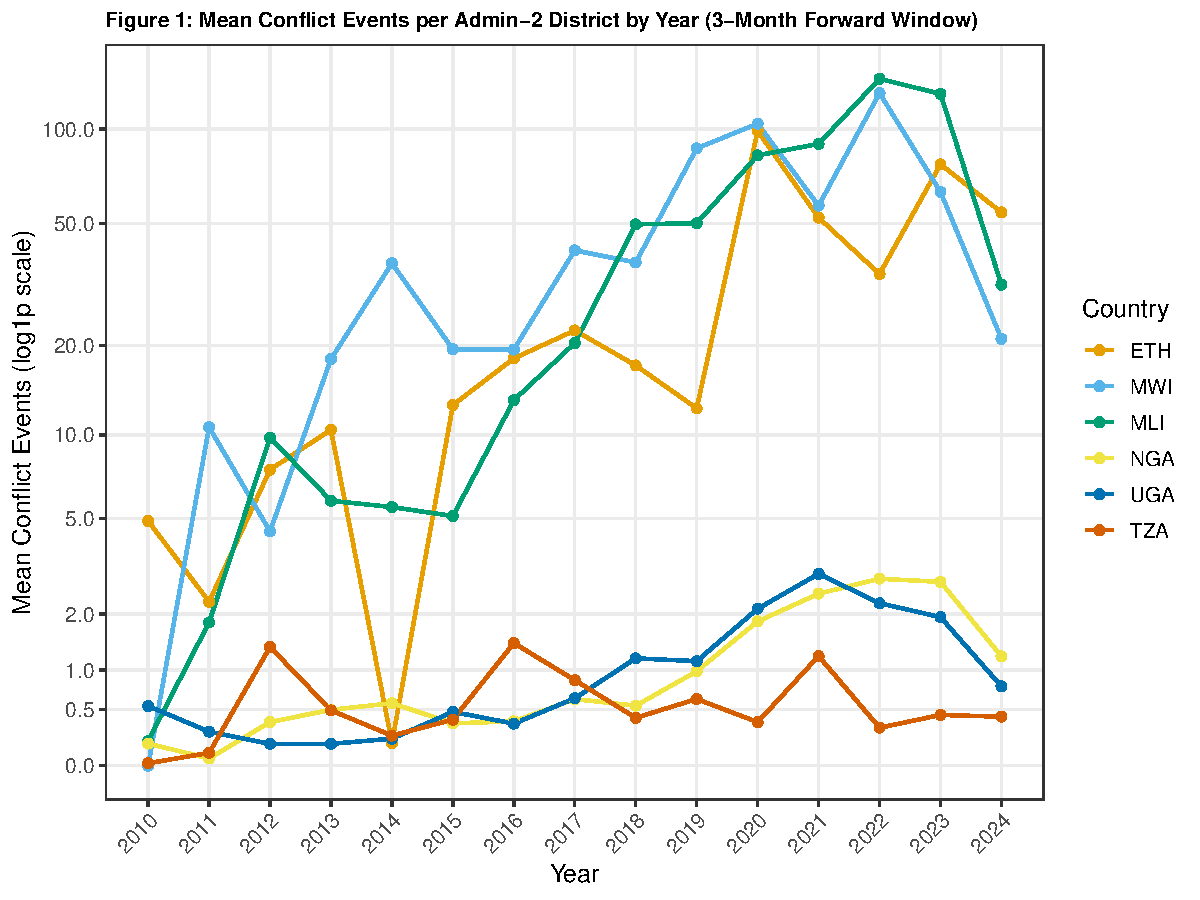
\includegraphics[width=0.90\textwidth]{figures/fig1_conflict_timeseries.pdf}
  \caption{Mean Conflict Events per Admin-2 District by Year (3-Month Forward Window)}
  \label{fig:conflict_timeseries}
  \footnotesize{Note: y-axis is on a log(1+x) scale to accommodate the large differences in mean conflict rates across countries. Each point represents the mean number of ACLED events recorded in the 3-month post-harvest window across all Admin-2 districts in a given country-year.}
\end{figure}

\subsection{Agricultural Survey Data (LSMS-ISA)}

Ground-truth yield observations for model training are drawn from nationally representative Living Standards Measurement Study -- Integrated Surveys on Agriculture (LSMS-ISA), a programme of household surveys conducted by the World Bank in collaboration with national statistical offices \citep{WorldBank_LSMS}. LSMS-ISA surveys provide detailed plot-level information on crop production, cultivated area, input use, and harvest outcomes, enabling the construction of plot-level yield estimates (kg/ha) for the primary food crops.

Survey coverage is limited both temporally and spatially. Each country contributes two to four survey waves, typically spaced two to three years apart, covering a subset of enumeration areas. The six countries in the analysis---Ethiopia, Malawi, Mali, Nigeria, Tanzania, and Uganda---all have at least two LSMS-ISA waves from which maize yield observations can be extracted. These survey observations serve exclusively as training data for the yield prediction models; they are not used directly as the regressor in the conflict panel, given their sparse and spatially unrepresentative coverage.

\subsection{Satellite and Environmental Data}

Satellite and environmental inputs for yield prediction are obtained from publicly available remote-sensing and climate reanalysis products, harmonised to a consistent spatial grid and temporal frequency. The following feature classes are used:

\textbf{Vegetation indices:} EVI (Enhanced Vegetation Index), NDVI (Normalised Difference Vegetation Index), and GCVI (Green Chlorophyll Vegetation Index), derived from MODIS or equivalent optical sensors. These indices proxy for canopy greenness, photosynthetic activity, and biomass, and are strongly correlated with crop growth and yield across a variety of crops and environments \citep{BurkeLobell2017}.

\textbf{Thermal stress indicators:} Growing Degree Days (GDD) and Killing Degree Days (KDD) computed from daily maximum and minimum temperature data. GDD accumulate heat units conducive to crop development, while KDD capture exposure to temperatures above critical thresholds that cause yield loss \citep{Schlenker_Roberts2009}.

\textbf{Temperature:} Monthly maximum and minimum temperature from reanalysis products (ERA5 or equivalent), used as direct inputs and to construct GDD and KDD.

All features are computed as monthly values and then aggregated into seasonal composites aligned to each survey point's mode harvest month. Twelve-month lag features (lags 0--11 relative to harvest) capture the full crop-development cycle. Seasonal aggregates are constructed for the growing season (lags 3--6), peak season (lags 4--5), near-harvest period (lags 0--2), and pre-season (lags 7--11), along with trend features (lag 3 minus lag 0) to capture within-season trajectories.

\textit{Known limitation:} Precipitation and soil moisture data are absent from the satellite extract used in this paper (100\% missing in the source parquet file). After imputation, these features are constant and contribute no predictive information. All observations are flagged as \texttt{precip\_missing = TRUE}. The absence of precipitation may attenuate model performance, particularly in rain-fed agricultural systems where water availability is the primary yield constraint. This limitation is acknowledged and its implications for inference are discussed in Section~\ref{sec:results}.

\subsection{Population Data}

District-level population counts by year are drawn from gridded population datasets aggregated to Admin-2 boundaries, covering the period 2010--2020. Values for 2021--2024 are carried forward from the 2020 observation, as consistent gridded population data extending beyond 2020 are not available for all countries. Population enters the regression as the natural log of total district population, $\log(\text{pop}_{it})$, and serves as a time-varying control for the size of the at-risk population within each district.

\subsection{Summary Statistics}

Table~\ref{tab:sumstats} reports panel-level summary statistics for the key variables used in the regression analysis.

\begin{table}[H]
\centering
\caption{Summary Statistics --- Full Panel}
\label{tab:sumstats}
\begin{threeparttable}
\begin{tabular}{lrrrrrr}
\toprule
Variable & N & Mean & SD & Min & Median & Max \\
\midrule
Conflict events (3-month)  & 13,890 & 6.3  & 50.9 & 0    & 0    & 1,944 \\
Conflict events (6-month)  & 13,890 & 11.9 & 94.0 & 0    & 0    & 3,608 \\
Conflict events (12-month) & 13,890 & 23.1 & 175.4 & 0   & 0    & 6,736 \\
Any conflict (binary, 3mo) & 13,890 & 0.16 & 0.37 & 0    & 0    & 1     \\
Fatalities (3-month)       & 13,890 & 13.9 & ---  & 0    & 0    & ---   \\
Log pred. yield (kg/ha)    & 13,890 & 6.67 & 0.39 & 5.62 & 6.72 & 7.55  \\
Predicted yield (kg/ha)    & 13,890 & 877  & 335  & 275  & 826  & 1,895 \\
Log population             & 13,890 & ---  & ---  & ---  & ---  & ---   \\
\bottomrule
\end{tabular}
\begin{tablenotes}
\small
\item Note: Log predicted yield is the natural log of ML-predicted maize yield (kg/ha). All conflict windows are 3-, 6-, and 12-month forward windows following the estimated district harvest month. 84.2\% of district-years record zero conflict events in the 3-month window.
\end{tablenotes}
\end{threeparttable}
\end{table}

\begin{figure}[H]
  \centering
  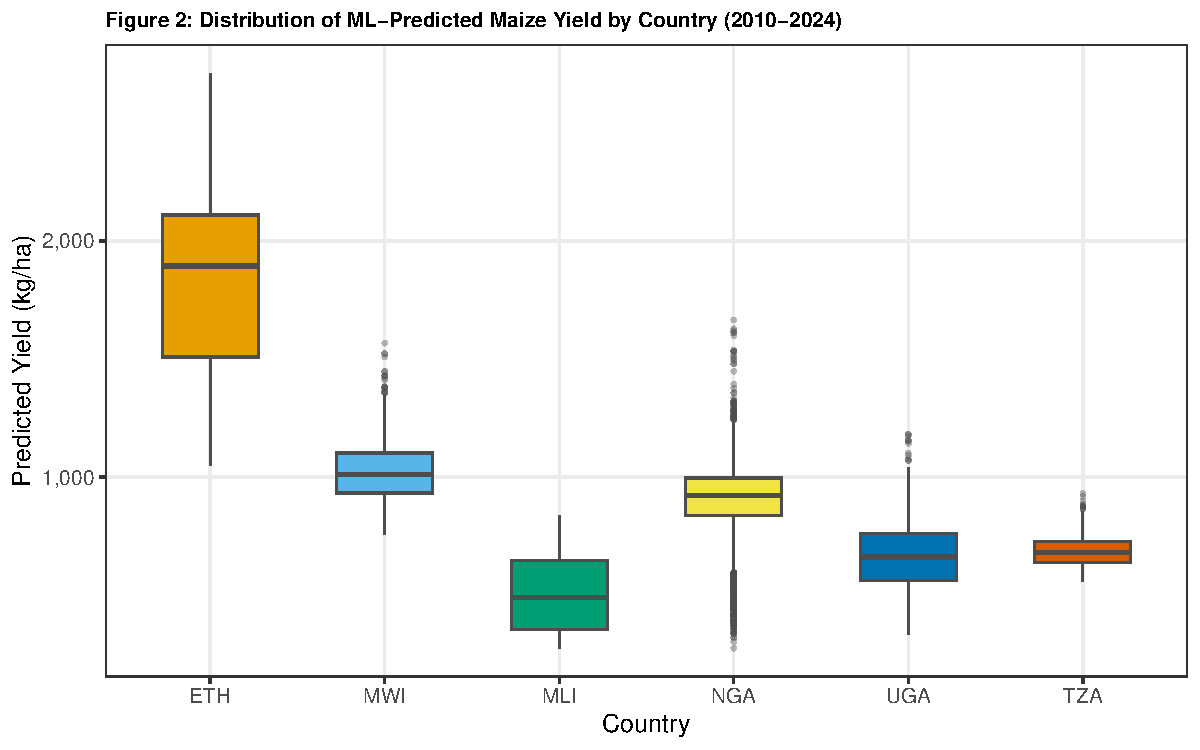
\includegraphics[width=0.90\textwidth]{figures/fig2_yield_distribution.pdf}
  \caption{Distribution of ML-Predicted Maize Yield by Country (2010--2024)}
  \label{fig:yield_distribution}
  \footnotesize{Note: Boxplots show the distribution of ML-predicted maize yield (kg/ha) across Admin-2 district-years. Box covers interquartile range; whiskers extend to 1.5$\times$IQR. ETH = Ethiopia; MWI = Malawi; MLI = Mali; NGA = Nigeria; UGA = Uganda; TZA = Tanzania.}
\end{figure}
